\section{Carga y Materia}

Todo lo que nos rodea, como una pelota, el aire, una planta o nuestro propio cuerpo, está formado por átomos. Los átomos, a su vez, están compuestos por tres tipos de partículas: protones, neutrones y electrones. Los protones y neutrones se encuentran en el núcleo del átomo, mientras que los electrones se mueven alrededor en la corteza. Los protones tienen carga positiva, los electrones carga negativa, y los neutrones no tienen carga. 

Esta estructura corresponde a un modelo atómico, que es una representación que nos ayuda a entender cómo está compuesto un átomo y cómo se comporta. A lo largo del tiempo han existido distintos modelos atómicos, pero uno de los más conocidos es el modelo de Bohr. Según este modelo, los electrones giran alrededor del núcleo en órbitas circulares, cada una con un nivel de energía específico. Cuando un electrón cambia de órbita, absorbe o emite energía en forma de luz. La figura \ref{fig_modelo_atomico} muestra una representación del átomo de Helio.

La carga elemental \(e\) es la cantidad más pequeña de carga eléctrica libre que se conoce en la naturaleza. Es la carga que poseen los protones y electrones, pero con signo opuesto:
\begin{itemize}
  \item Electrón: \( -e = -\qty{1.602e-19}{\coulomb}\)
  \item Protón: \( +e = \qty{1.602e-19}{\coulomb} \)
\end{itemize}
\begin{marginfigure}
  \centering
  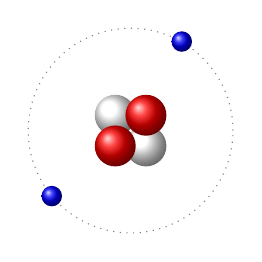
\begin{tikzpicture}[scale=1.3]
    \shade[ball color=white] (-.15,.15) circle (.2);
    \shade[ball color=white] (.15,-.15) circle (.2);
    \shade[ball color=red] (-.15,-.15) circle (.2);
    \shade[ball color=red] (.15,.15) circle (.2);
    \draw[dotted,gray] (0,0) circle (1);
    \shade[ball color=blue] (.5,.87) circle (.1);
    \shade[ball color=blue] (-.77,-.64) circle (.1);
  \end{tikzpicture}
  \caption{Representación del modelo básico de un átomo.}
  \label{fig_modelo_atomico}
\end{marginfigure}

La carga elemental es fundamental porque todas las cargas eléctricas observadas en la naturaleza son múltiplos enteros de \( e \). Es decir, cualquier carga presente en un objeto es el resultado de un exceso o déficit de electrones. Este principio se conoce como la ley de conservación de la carga eléctrica, y establece que la carga eléctrica no se crea ni se destruye, solo se transfiere de un cuerpo a otro. Un objeto es eléctricamente neutro cuando tiene igual número de ambos. Si un objeto adquiere carga negativa, significa que ha ganado electrones, y si adquiere carga positiva, significa que ha perdido electrones. Cuando un objeto se carga, no se están creando nuevas cargas, sino que se están moviendo electrones de un cuerpo a otro. Por ejemplo: en la electrización por frotamiento, un material transfiere electrones a otro, dejando uno cargado positivamente y el otro negativamente.

Denominaremos con la letra \( Q \) o \( q \) a la carga eléctrica de un objeto. La carga se mide en Coulombs (\unit{\coulomb}). Un Coulomb es una cantidad de carga muy grande, por lo que en la práctica se utilizan submúltiplos como el milicoulomb (\unit{\milli\coulomb}) o el microcoulomb (\unit{\micro\coulomb}).
